% Block-NCM, paper 1. Build: pdflatex blockncm && pdflatex blockncm   (figures: python scripts/make_figures.py)
% Every number is from RESULTS.md; the section of RESULTS.md is named in a comment next to each table.
\documentclass[10pt,twocolumn]{article}
\usepackage[margin=0.75in,columnsep=0.25in]{geometry}
\usepackage[T1]{fontenc}
\usepackage{lmodern}
\usepackage{amsmath,amssymb}
\usepackage{booktabs}
\usepackage{graphicx}
\usepackage{xcolor}
\usepackage{enumitem}
\usepackage{caption}
\usepackage[hidelinks]{hyperref}
\captionsetup{font=small,labelfont=bf}
\setlist{nosep,leftmargin=*}
\newcommand{\seam}{\textcolor{red!70!black}{\,$\Vert$\,}}
\definecolor{ours}{HTML}{1f77b4}

\title{\textbf{Block-NCM: Long Stories in a Constant Number of Parallel Passes}}
\author{Rishab Gupta\\ \small BITS Pilani, Dubai Campus}
\date{November 2026}

\raggedbottom
\begin{document}
\maketitle

\begin{abstract}
Next-Concept Models (NCM) generate a 128-token chunk of text coarse to fine in 11 parallel passes, one per level of
a residual code hierarchy. Extending them to longer outputs has two obvious options. Generating chunks one after
another multiplies the number of sequential passes by the number of chunks. Letting every level attend across all
chunks keeps 11 passes but, as we show, fits the trained length and collapses beyond it. We propose
\emph{Block-NCM}: the first $G$ coarse levels form a story plan shared by all chunks, the remaining levels are
local to each chunk, and a small \emph{halo} lets local levels see a few positions of each neighbour. Any number of
chunks still takes 11 passes. Fine-tuned from the released TinyStories NCM on 512-token stories, Block-NCM writes a
story 16.5$\times$ faster than a smaller (68.5M-parameter) autoregressive (AR) model at batch size 1 on the same GPU
(3.2$\times$ at batch 32). Its batch-1 latency stays at about 0.37\,s from 256 to 1024 tokens, while generating the
chunks one after another becomes up to 9.4$\times$ slower. At the trained length it is within 0.5--2.4 genPPL of fully global attention, with
better NLL. At 1.5$\times$ the trained length fully global attention degrades from 18.7 to 31.3 genPPL over three
seeds, while Block-NCM with $G{=}3$ stays at 21.2. A matched per-chunk test shows the collapse starts in the first
chunk and grows with the number of global levels. Block-NCM's text remains about 2$\times$ worse than the AR model's
by genPPL, a gap mostly inherited from base NCM; we leave quality to follow-up work.
\end{abstract}

% =====================================================================
\section{Introduction}

Autoregressive (AR) language models need one sequential forward pass per generated token. Next-Concept Models
(NCM)~\cite{ncm} instead encode a chunk of text into a hierarchy of residual vector-quantised codes and generate the
hierarchy level by level, all positions of a level in parallel. The released TinyStories model produces 128 tokens
in 11 sequential passes\footnote{The NCM paper counts 12 function evaluations. Level 0 (one code) is drawn from a
stored unigram table, not by a transformer pass, so we count 11.}, and its authors report it to be 10--31$\times$
faster than diffusion language models at comparable quality on three benchmarks~\cite{ncm}. Its tokenizer and
generator, however, see only 128 tokens at a time. Here, ``long'' means longer than that window: we train on 512
tokens and test up to 768.

This paper asks how to keep NCM's small, fixed number of passes when the output is several chunks long. Two simple
answers exist (Figure~\ref{fig:arch}):
\begin{itemize}
  \item \textbf{B1, chunks in sequence:} generate chunk $m$ conditioned on chunks $1..m{-}1$. Quality can be good,
        but the number of passes grows to $11M$ for $M$ chunks, giving up NCM's advantage.
  \item \textbf{B2, fully global:} treat the $M$ chunks as one long sequence at every level. Still 11 passes, but
        every level attends across $M\times$ more positions.
\end{itemize}
We find that B2 works at the trained length and \emph{collapses} at longer lengths (Section~\ref{sec:length}).
Block-NCM sits between the two: only the coarse levels, which carry topic and characters, attend across chunks.

\paragraph{Contributions.}
\begin{enumerate}
  \item \textbf{Block-NCM}, a chunked NCM whose coarse levels form a shared plan and whose fine levels are local
        with a small halo. It takes 11 sequential passes for any number of chunks (Section~\ref{sec:method}).
  \item \textbf{Measured speed}: 16.5$\times$ faster than an AR model at batch 1 and 3.2$\times$ at batch 32 on the
        same GPU, and batch-1 latency that stays flat from 256 to 1024 tokens on our GPU, unlike chunks generated
        in sequence (2.1--9.4$\times$ slower over the same range) (Section~\ref{sec:speed}).
  \item \textbf{A quality--robustness trade-off in $G$}: more global levels give better text at the trained length
        and worse text beyond it, with fully global attention at the extreme. A matched per-chunk test shows the
        failure comes from cross-chunk attention and starts in the first chunk (Section~\ref{sec:length}).
  \item \textbf{A record of what failed}: conditioning corruption is required to fine-tune NCM at all, and four
        other ideas did not work (Appendix~\ref{sec:failures}).
\end{enumerate}

% =====================================================================
\section{Background: Next-Concept Models}
\label{sec:background}

NCM~\cite{ncm} pairs a VQ-VAE tokenizer~\cite{vqvae} with a generator. The tokenizer maps 128 tokens (BPE with a
vocabulary of 8,192) to a latent sequence and quantises it with residual vector quantisation~\cite{soundstream} over levels of increasing
length. In the released TinyStories model, a single position at level 0 is followed by 11 target levels of length
$(8,16,24,32,40,52,64,76,92,108,128)$: 641 codes per chunk. Level $k$ refines the reconstruction left by levels
$<k$, so coarse levels hold the gist and fine levels hold token-level detail; the last level cannot be dropped
without losing tokens (Appendix~\ref{sec:probe}).

The generator is a transformer (89.0M parameters) that predicts all codes of level $k$ in one pass, given the running reconstruction
from levels $<k$. Generating a chunk therefore takes 11 passes regardless of its length. During training the
generator's conditioning codes are partly replaced by random codes from the same codebook (\emph{conditioning
corruption}, mean rate 0.5), which makes it robust to its own sampling errors~\cite{ncm}. We found this step
essential for fine-tuning (Appendix~\ref{sec:failures}).

% =====================================================================
\section{Block-NCM}
\label{sec:method}

\begin{figure*}[t]
  \centering
  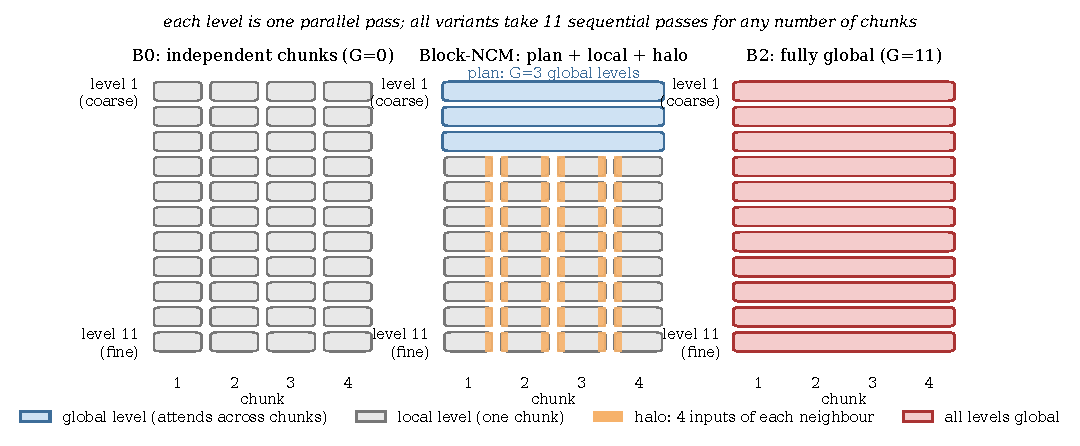
\includegraphics[width=0.92\textwidth]{figures/fig_architecture.pdf}
  \caption{Which positions each level attends to, for $M{=}4$ chunks. Each row is one level and one parallel pass.
  B0 never connects chunks; B2 connects them at every level. Block-NCM connects them only at the first $G$ levels
  (the plan) and lets local levels see $h{=}4$ input positions of each neighbouring chunk (halo). All three take
  11 sequential passes for any $M$; B1 (not shown) would take $11M$.}
  \label{fig:arch}
\end{figure*}

A story of $M$ chunks is encoded chunk by chunk with the frozen tokenizer, giving $M$ copies of the 11-level
hierarchy. Generation runs level by level as in NCM, with all chunks in the batch, so the number of sequential passes
stays at 11. What changes is the attention pattern at each level (Figure~\ref{fig:arch}).

\paragraph{Plan levels ($k\le G$).} The codes of all $M$ chunks at level $k$ form one sequence, with a learned chunk
embedding added to each position. Every position attends to every chunk. These levels are short (8, 16 and 24
positions per chunk for $G{=}3$), so cross-chunk attention is cheap. They decide what each chunk is about.

\paragraph{Local levels ($k>G$).} Each chunk is its own sequence and also attends to the plan levels' keys and
values. Those are computed once and cached for all local levels, which halves training time without changing the
result (losses equal to within $8{\times}10^{-7}$). Local levels hold 592 of the 641 codes per chunk for $G{=}3$.

\paragraph{Halo.} A local level of chunk $m$ also attends to the level's \emph{inputs} at the last $h$ positions
of chunk $m{-}1$ and the first $h$ positions of chunk $m{+}1$. These inputs come from coarser levels that are
already generated, so the halo adds no sequential pass. It targets the seams, where a sentence must run on from one
chunk into the next. It adds $2h$ positions per chunk per local level, about 10\% compute for $h{=}4$.

\paragraph{Special cases.} $G{=}0$ without halo is \textbf{B0} (independent chunks). $G{=}11$ is \textbf{B2}
(fully global). We study $G\in\{3,5,6\}$ with $h\in\{2,4,8\}$.

\paragraph{Training.} We fine-tune all generator weights of the released TinyStories NCM. Each step sees $M{=}4$
chunks of a story. The loss is the cross-entropy of every level's codes given the clean codes of the coarser levels,
with conditioning corruption on the inputs (rate falling linearly from 0.75 to 0.25 over levels; targets stay
clean). Padding codes after the end of a story are masked from all metrics.

% =====================================================================
\section{Experimental setup}
\label{sec:setup}

\paragraph{Data.} TinyStories~\cite{tinystories} as released with NCM (BPE-8192 tokenisation), stories longer than
384 tokens (4.7\% of the corpus):
125,723 training and 1,228 validation stories, cut to 512 tokens ($M{=}4$). Evaluation at $M{=}6$ (768 tokens)
uses models trained only on $M{=}4$.

\paragraph{Models.} B0, B2, and Block-NCM with $G{=}3$ or $G{=}5$ and halo $h{=}4$, all fine-tuned from the
released checkpoint with the same recipe: 1,500 steps of 8 stories, AdamW, lr $3{\times}10^{-5}$ with 200 warm-up
steps and cosine decay, gradient checkpointing. Main models are trained with three seeds. For B0, $G{=}3$ and B2,
one seed ran locally in bf16 on an RTX~5050 laptop GPU and two on Kaggle T4s in fp16; for $G{=}5$, all three ran
on Kaggle. A fourth $G{=}5$ run, trained locally, is reported separately: it matches the others at $M{=}4$ (19.4)
but reaches 25.2 at $M{=}6$. With it, the four-run means are 19.3 and 21.8. Local and Kaggle runs differ in
precision and in their encoding of the data, and we have not found the cause of this gap.

\paragraph{Metrics.}
\begin{itemize}
  \item \textbf{genPPL}: perplexity of generated text under GPT-2 Large~\cite{gpt2}, the NCM paper's protocol;
        2 sampling seeds $\times$ 256 unconditional samples, temperature 1.0, no top-$k$/top-$p$, text cut at the
        first end-of-text token. Lower is better.
  \item \textbf{Seam ratio}: genPPL of 64-token windows across a chunk boundary divided by genPPL of 64-token
        windows inside a chunk. Real text scores 1.01; an AR model's samples score 1.04.
  \item \textbf{NLL}: teacher-forced loss on all validation stories, padding masked, compared with a paired
        per-story bootstrap (1,000 resamples).
\end{itemize}

\paragraph{Reference points.} The released NCM scores 16.38 $\pm$ 0.22 genPPL on single 128-token chunks in our
reproduction (paper: 15.41~\cite{ncm}). As an AR reference we use TinyStories-33M~\cite{tinystories}, a GPT-Neo trained on
TinyStories with 68.5M parameters including embeddings; at 128 tokens it scores 9.68, close to the NCM paper's 88.6M AR baseline (8.89).

% =====================================================================
\section{Results}

\subsection{Speed}
\label{sec:speed}

\begin{figure}[t]
  \centering
  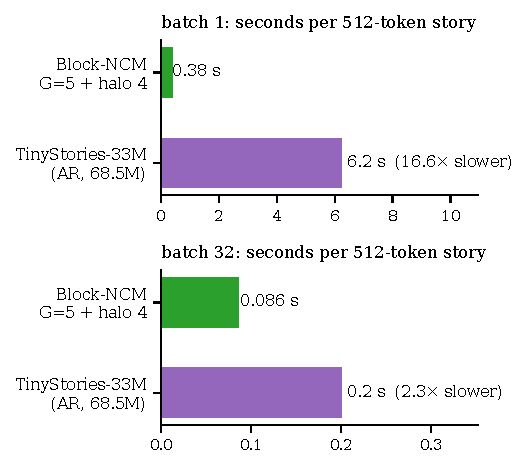
\includegraphics[width=\columnwidth]{figures/fig_speed.pdf}
  \caption{Wall-clock time on one RTX~5050 laptop GPU (8\,GB; median of 10 runs after 3 warm-ups; Block-NCM is
  $G{=}5$, $h{=}4$, and its time includes decoding codes to tokens). (a) Batch 1, stories of 2, 4 and 8 chunks.
  B1 is timed as $M$ single-chunk generations in sequence, a lower bound (see text); labels give B1's time over
  Block-NCM's. (b) 512-token stories; labels give AR's time over Block-NCM's. The AR model uses Hugging Face
  \texttt{generate} with a KV cache, sampling exactly 517 GPT-Neo tokens ($\approx$512 BPE tokens).}
  \label{fig:speed}
\end{figure}

\paragraph{Against an AR model.} Figure~\ref{fig:speed}b compares Block-NCM with TinyStories-33M generating the
same length. At batch 1, Block-NCM takes 0.38\,s per story and the AR model 6.20\,s: \textbf{16.5$\times$ faster}.
The ratio falls with batch size, to 10.8$\times$ at batch 8, 6.0$\times$ at 16 and \textbf{3.2$\times$ at 32}
(0.063 vs 0.202\,s per story). Block-NCM is compute-bound from batch 16, while the AR loop's time per batch stays at
6.0--6.5\,s from batch 1 to 32, so its per-token overhead is shared across the batch and AR would overtake
Block-NCM at some larger batch. Block-NCM's generator is larger than the AR model (89.0M against 68.5M
parameters), so the speed comes from making 11 passes instead of about 517, not from a smaller model.

\paragraph{Against chunks in sequence (B1).} B1 has no trained model of its own, but latency does not depend on the
weights, so we time it as $M$ single-chunk generations of the released NCM run one after another (11 passes each)
plus decoding. A real B1 would also attend to the text before each chunk, which makes every pass longer, so this
is a lower bound on its time. At batch 1 (Figure~\ref{fig:speed}a), Block-NCM's latency stays at 0.36--0.39\,s
from 256 to 1024 tokens, while B1's grows linearly from 0.80 to 3.56\,s: \textbf{2.1$\times$, 4.3$\times$ and
9.4$\times$ slower} for 2, 4 and 8 chunks (an earlier run gave 2.3$\times$, 4.8$\times$ and 7.8$\times$). At
batch 8 B1 is 2.1--3.3$\times$ slower. At batch 32 the two tie (1.0--1.1$\times$): both process the same number
of chunk positions per pass, and the GPU is saturated. Block-NCM's gain over B1 is latency, not throughput.

Three details matter for a fair comparison. First, the AR side uses unoptimised \texttt{generate} without CUDA
graphs or fused kernels, so the batch-1 ratio is an upper bound. At batch 1, AR timings varied between 6.2 and
8.1\,s across runs (laptop GPU clocks); we report the fastest. Second, the tokenizer's decoder must run with TF32 or fp16 matrix multiplies: in plain fp32 it hits a slow
path that takes 4.2\,s at batch 32. We run the code lookup in fp32 and the decoder in fp16, which matches the fp32
output on 99.96\% of tokens. Third, memory: with PyTorch's default allocator, Block-NCM at batch 32 reserved
8.6\,GiB for 512 tokens, although it allocated only 3.6\,GiB, and the excess spilled into system memory, which
slowed it by about 50\%. All timings use expandable allocator segments, which keep it at 3.8\,GiB. A 1024-token
batch of 32 does not fit in 8\,GB.

\paragraph{At 7B scale (estimate).} A roofline cost model with both models at 7B parameters on an H100
(Appendix~\ref{sec:cost}) predicts 26--27$\times$ lower batch-1 latency than an AR model for 2,048-token outputs,
with AR becoming cheaper per token from batch 31. The same model puts B1 about 2.3$\times$ slower than Block-NCM at
batch 1 at 2,048 tokens, less than we measure on the small model: at 7B a pass over all 16 chunks is compute-bound
and costs several single-chunk passes, whereas on the small GPU-underfilling model a pass over 8 chunks costs
about the same as a pass over one. Block-NCM processes about 5.4 positions per output token, so
high-throughput serving favours AR; the case for Block-NCM is low-batch, latency-bound generation. In this model
Block-NCM is about 5\% slower than B2, because halo positions add queries.

\subsection{Quality at the trained length}
\label{sec:quality}

% RESULTS.md: "Third seed of the main models"
\begin{table}[t]
\centering
\small
\caption{Main models at the trained length ($M{=}4$, 512 tokens) and at $M{=}6$ (768 tokens, never trained).
genPPL: mean $\pm$ sd over three training seeds; seam ratio: mean. NLL: the seed-2 runs, which share one
encoding of the validation set (NLL is comparable only within one encoding); $\Delta$ vs B2 with 95\% bootstrap
CI. B2 has the worst NLL on all three seeds.}
\label{tab:main}
\setlength{\tabcolsep}{2.4pt}
\resizebox{\columnwidth}{!}{%
\begin{tabular}{@{}lcccc@{}}
\toprule
 & B0 & \textcolor{ours}{G3+h4} & \textcolor{ours}{G5+h4} & B2 \\
\midrule
genPPL, $M{=}4$ & 24.2{\tiny$\pm$0.3} & 21.1{\tiny$\pm$0.3} & 19.2{\tiny$\pm$0.3} & \textbf{18.7}{\tiny$\pm$0.3} \\
seam ratio, $M{=}4$ & 1.49 & 1.20 & 1.14 & \textbf{1.12} \\
genPPL, $M{=}6$ & 23.8{\tiny$\pm$0.1} & 21.2{\tiny$\pm$0.6} & \textbf{20.6}{\tiny$\pm$0.5} & 31.3{\tiny$\pm$2.1} \\
seam ratio, $M{=}6$ & 1.50 & 1.19 & 1.15 & 1.14 \\
\midrule
NLL & 1.6151 & 1.5993 & \textbf{1.5928} & 1.6327 \\
$\Delta$NLL vs B2 & $-$0.017 & $-$0.033 & $\mathbf{-0.040}$ & -- \\
\quad 95\% CI & {\scriptsize[$-$.018, $-$.016]} & {\scriptsize[$-$.034, $-$.032]} & {\scriptsize[$-$.041, $-$.039]} & \\
NLL, chunk 4 & 1.686 & \textbf{1.666} & 1.667 & 1.744 \\
\bottomrule
\end{tabular}}
\end{table}

Table~\ref{tab:main} shows the main models at the trained length. \textbf{B2 writes the best text at $M{=}4$}
(18.7 genPPL), with Block-NCM $G{=}5$ 0.5 behind and $G{=}3$ 2.4 behind. Seams are close to tied (1.12 vs 1.14), and
both are near the 1.04 that AR samples reach without any seams. B0, which never connects chunks, has the worst text
and seams (24.2, 1.49) and visibly loses track of its characters (Figure~\ref{fig:samples}).

\textbf{B2 has the worst NLL of all models}, worse even than B0, on every seed (each seed is compared within its
own encoding). Both Block-NCM models beat it with
non-overlapping confidence intervals. B2's loss is concentrated on the fine levels (6--11) and on chunk 4: global
attention at the finest levels hurts teacher-forced prediction, plausibly because the released model never saw
positions beyond 128 at those levels. Teacher-forced NLL and free generation rank B2 differently, so we report both.

\begin{figure}[t]
\small
\setlength{\fboxsep}{4pt}
\fbox{\parbox{0.95\columnwidth}{\textbf{B0} ($G{=}0$)\quad \dots One day, Sam goes to the park with his mom. He sees
a girl with a brown helmet. \dots ``Hey, my my car is faster than yours!'' Sam says, pointing to his bike.\seam
Okay, go,'','' Ben said. ``I will be careful if you want.'' They climbed stairs to the other side of the slide.
\dots}}\\[3pt]
\fbox{\parbox{0.95\columnwidth}{\textbf{\textcolor{ours}{Block-NCM}} ($G{=}3$, $h{=}4$)\quad \dots Lila jumps in the
puddles. But it is too wet and slippery. She comes off and hits her hand on the ground. ``Ow, ow, Billy!'' Lila
cries, rubbing her arm\seam. Ben runs to the puddle and hugs her. He lets Sara go away. \dots}}\\[3pt]
\fbox{\parbox{0.95\columnwidth}{\textbf{B2} ($G{=}11$)\quad \dots He jumped off and bit her hand. ``Ow, ow, ow! That
hurts!'' Lila cried, poking her finger.\seam ``Ow, that hurts!'' Ben said. ``You hurt!'' Lila ran and to him to
the bush. \dots}}
\caption{Text on either side of the first chunk boundary (\seam), verbatim including errors. Each excerpt is from
sample 1 of the model's evaluation file (same sampling seed and index for all three; samples 0 and 1 are the first
two that reach chunk 4). B0 switches to different characters at the seam. Block-NCM continues the sentence
across the seam but introduces a new name (Sara); B2 keeps both characters.}
\label{fig:samples}
\end{figure}

\subsection{Beyond the trained length}
\label{sec:length}

\begin{figure*}[t]
  \centering
  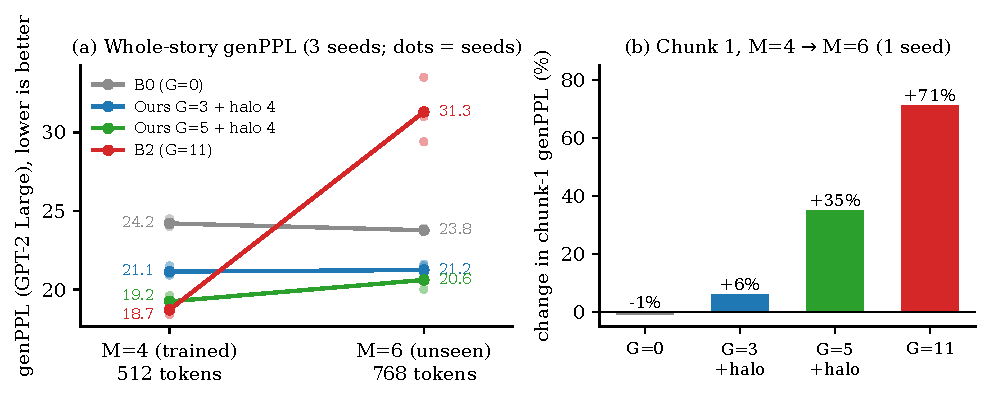
\includegraphics[width=0.86\textwidth]{figures/fig_tradeoff.pdf}
  \caption{(a) Whole-story genPPL at the trained length and at 1.5$\times$ it, for three training seeds. B2
  degrades on every seed (19.0$\to$33.5, 18.4$\to$31.0, 18.7$\to$29.4); Block-NCM $G{=}3$ does not move.
  (b) Matched test: change in the genPPL of chunk 1 when the model is asked for 6 chunks instead of 4. Chunk 1
  covers tokens 0--127, so story length cannot explain the change.}
  \label{fig:tradeoff}
\end{figure*}

At $M{=}6$, 1.5$\times$ the trained length, the ranking flips (Figure~\ref{fig:tradeoff}a). B2 degrades from 18.7
to 31.3 genPPL, replicated on all three training seeds, and to 57.3 at sampling temperature 0.8. Block-NCM $G{=}3$
goes from 21.1 to 21.2 and $G{=}5$ from 19.2 to 20.6. B0, with no cross-chunk attention, does not degrade either.
Among one-seed runs without halo, the same pattern holds: $G{=}6$ goes from 19.6 to 30.7 and $G{=}5$ from 20.0 to 23.8,
while $G{=}3$ holds (21.8).

\paragraph{Ruling out story length.} Whole-story genPPL at $M{=}6$ is confounded: most samples end their story within
four chunks, as the training stories do, and models that keep writing are scored on more text. Two checks remove
this. First, scoring only samples longer than 4.5 chunks keeps the ranking: $G{=}3$ 22.5, $G{=}5$ 30.8, B2 49.8
(one seed). Second, a \emph{matched per-chunk test} compares the same positions under both lengths: chunk $m$ of
$M{=}4$ samples against chunk $m$ of $M{=}6$ samples, each scored by GPT-2 Large given the story before it
(Figure~\ref{fig:chunks}). B2's chunks 1--4 are all 58--71\% worse when it generates 6 chunks. Its \emph{first}
chunk goes from 20.6 to 35.3 genPPL. Chunk 1 covers the same tokens 0--127 under both lengths, and all chunks are
generated together, level by level, so the damage cannot come from errors piling up over a long story. It comes
from attention across more chunks than in training, and it grows with the number of levels that attend across
chunks: $-1\%$ for $G{=}0$, $+6\%$ for $G{=}3$, $+35\%$ for $G{=}5$, and $+71\%$ for B2
(Figure~\ref{fig:tradeoff}b).

\begin{figure}[t]
  \centering
  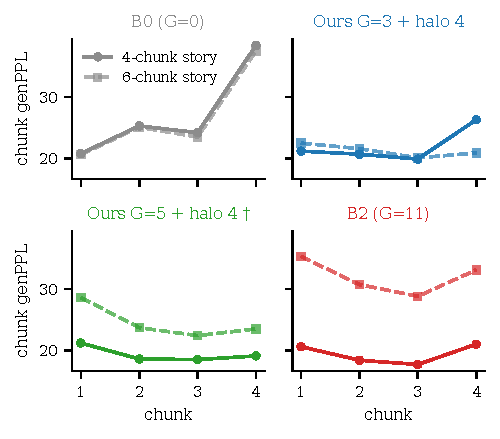
\includegraphics[width=\columnwidth]{figures/fig_chunks.pdf}
  \caption{Matched per-chunk genPPL: each chunk scored given the story before it, in 4-chunk stories (solid) and
  6-chunk stories (dashed), temperature 1.0, one training seed, 430--512 samples per point. \dag~This $G{=}5$ run is
  the weakest of four seeds (whole-story $M{=}6$ genPPL 25.2 vs 20.0--21.0 for the other three).}
  \label{fig:chunks}
\end{figure}

\paragraph{Interpretation.} Attention that spans all chunks fits the number of chunks it was trained on. When
it must cover more chunks, every chunk generated under it suffers. Block-NCM confines cross-chunk attention to
a few short coarse levels and leaves most of the model local, so most of the model never sees the change in length.
Two concrete causes are plausible, and we have not separated them. First, the learned chunk embeddings of chunks 5
and 6 are never trained and stay at their zero initialisation. Second, cross-chunk levels see rotary positions
beyond those seen in fine-tuning. Every model receives the untrained embeddings, and B0, which never attends across
chunks, does not degrade; so both causes would act through cross-chunk attention, consistent with the dependence
on $G$.
The choice of $G$ is a trade-off: $G{=}5$ is 1.9 genPPL better than $G{=}3$ at the trained length, and $G{=}3$ is
nearly unaffected by length. No model extends gracefully, though: text beyond token 512 scores worse than text within
it for all of them.

\subsection{Ablations}
\label{sec:ablations}

% RESULTS.md: Milestone 5, Milestone 5b, Sampling temperature, quality probe 2026-11-20
\begin{table}[t]
\centering
\small
\caption{Ablations at $M{=}4$ (one training seed). genPPL and seam ratio; $M{=}6$ genPPL in the last column.}
\label{tab:ablation}
\setlength{\tabcolsep}{4pt}
\begin{tabular}{@{}lccc@{}}
\toprule
variant & genPPL & seams & $M{=}6$ \\
\midrule
B0 ($G{=}0$) & 24.1 & 1.52 & 23.7 \\
$G{=}3$, no halo & 22.0 & 1.39 & 21.8 \\
$G{=}3$, $h{=}2$ & 21.4 & 1.22 & 21.1 \\
$G{=}3$, $h{=}4$ & 21.0 & 1.19 & 21.5 \\
$G{=}3$, $h{=}8$ & 20.4 & 1.17 & 20.4 \\
$G{=}5$, no halo & 20.0 & 1.26 & 23.8 \\
$G{=}5$, $h{=}4$ & 19.1 & 1.14 & 20.0 \\
$G{=}6$, no halo & 19.6 & 1.22 & 30.7 \\
$G{=}6$, $h{=}4$ & 18.7 & 1.12 & 23.6 \\
B2 ($G{=}11$) & 19.0 & 1.17 & 33.5 \\
\midrule
$G{=}5$, $h{=}4$ (local run) & 19.4 & 1.17 & 25.2 \\
$G{=}3$, $h{=}4$ + plan search (8) & 20.0 & 1.21 & -- \\
$G{=}5$, $h{=}4$ + plan search (8)$^\ast$ & 17.1 & 1.16 & -- \\
\bottomrule
\multicolumn{4}{@{}p{0.95\columnwidth}@{}}{\footnotesize Upper block: halo and $G$ sweeps. B0, B2, $G{=}3$ with no
halo or $h{=}4$, and $G{=}5,6$ with no halo are local runs; $h{=}2,8$ and $G{=}5,6$ with $h{=}4$ ran on Kaggle.
Lower block: plan search applied to the local runs listed just above it. $^\ast$Entropy 4.36$\to$4.32, length
413$\to$406 tokens.}
\end{tabular}
\end{table}

\paragraph{Halo.} Without halo, the plan alone closes only 38\% of the B0$\to$B2 seam gap ($G{=}3$: 1.39). A halo of
4 positions brings the seam ratio to 1.19, 95\% of the gap, and gives the best NLL of the local one-seed runs
(Appendix~\ref{sec:failures}). Wider halos help a little more ($h{=}2$ vs $h{=}8$, both on Kaggle;
Table~\ref{tab:ablation}). With halo, the three Kaggle $G{=}5$ seeds hold at $M{=}6$ (20.0--21.0), where the local
run without halo reached 23.8. That comparison crosses platforms, though, and the local $G{=}5$ run with halo
reached 25.2, so whether halo repairs extrapolation for $G{=}5$ is not settled. For $G{=}6$ it does not (23.6).

\paragraph{Number of plan levels.} At $M{=}4$, genPPL improves steadily with $G$; at $M{=}6$, $G\ge6$ degrades even
with halo. $G{=}3$ or $G{=}5$ with halo are the useful operating points.

\paragraph{Plan search.} Sampling 8 plans per story and keeping the one the model scores highest, then running the
local levels once, improves genPPL from 21.0 to 20.0 for $G{=}3$ and from 19.4 to 17.1 for $G{=}5$ (local run;
entropy 4.36$\to$4.32, length 413$\to$406 tokens). It costs only extra plan-level passes, about 1.3$\times$ the
latency for $G{=}3$.

\paragraph{Temperature.} Sampling at temperature 0.8 lowers genPPL by about 23\% for every model at $M{=}4$ and keeps
the ranking. It makes failure beyond the trained length worse: B2 goes to 57.3 at $M{=}6$.

\subsection{Quality against AR and base NCM}
\label{sec:gap}

% RESULTS.md: "AR reference vs base NCM vs Block-NCM"
\begin{table}[t]
\centering
\small
\caption{Quality reference points (genPPL, GPT-2 Large, temperature 1.0).}
\label{tab:gap}
\setlength{\tabcolsep}{4pt}
\begin{tabular}{@{}lcc@{}}
\toprule
 & 128 tokens & 512 tokens \\
\midrule
real TinyStories text & 9.67~\cite{ncm} & 6.1$^a$ \\
AR, TinyStories-33M & 9.68 & 9.9$^b$ \\
released NCM & 16.4 & 14.4$^c$ \\
Block-NCM $G{=}5$+$h{=}4$ & -- & 19.2 \\
\quad + plan search (local run) & -- & 17.1 \\
\bottomrule
\multicolumn{3}{@{}p{0.95\columnwidth}@{}}{\footnotesize $^a$Long stories only. $^b$End-of-text blocked for the
first 400 tokens: 457 tokens on average, against about 425 for Block-NCM samples, which stop at their first
end-of-text token. $^c$Four independent 128-token openings, not one story: seam ratio 1.25, entropy 4.80; each fresh opening
scores well under GPT-2 Large.}
\end{tabular}
\end{table}

Block-NCM's text is about 2$\times$ worse than the AR model's by genPPL (19.2 vs 9.9 at 512 tokens;
Table~\ref{tab:gap}). Most of this gap is inherited: the released NCM is already 1.7$\times$ behind the AR model on
single chunks (16.4 vs 9.7), as in the NCM paper's own comparison (15.41 vs 8.89)~\cite{ncm}. Fine-tuning adds about
4 genPPL per chunk (chunk 1 scores about 21 for every model). About 1.6 of that is a change of style: stories longer
than 384 tokens never open with ``Once upon a time'' (0\% vs 58\% of all stories), and GPT-2 Large scores real
long-story openings 1.10$\times$ higher than all openings. The remaining $\approx$2.4 comes from fine-tuning on the
small long-story subset, not from the recipe itself: trained on stories of all lengths, the same recipe reaches 17.0
on single chunks, close to the released model (Appendix~\ref{sec:failures}). Part of the AR gap is also style, since
TinyStories-33M writes mostly ``Once upon a time'' openings.

% =====================================================================
\section{Related work}

\paragraph{Parallel and non-autoregressive text generation.} Non-autoregressive translation~\cite{gu2018nat} and
iterative mask-predict decoding~\cite{maskpredict, maskgit} generate many tokens per pass. Discrete diffusion language
models~\cite{sedd, mdlm} refine all positions over many steps; block diffusion~\cite{bd3lm} generates blocks in
sequence with diffusion inside each block, which corresponds to our B1. NCM~\cite{ncm} generates coarse to fine over
a residual code hierarchy~\cite{vqvae, soundstream} in a small fixed number of passes. Residual quantisation also
underlies RQ-Transformer~\cite{rqtransformer}, which predicts each position's stack of codes autoregressively
across positions; NCM instead generates one level at a time for all positions. Block-NCM extends NCM beyond its
tokenizer's 128-token window without adding passes.

\paragraph{Planning for parallel long-form generation.} Writing a plan first and the text second is an old idea.
Progressive generation~\cite{progressive} expands content keywords into a full passage over several stages, and
PLANNER~\cite{planner} generates paragraph-level latent embeddings coarse to fine with diffusion, then decodes
them with an AR model. Skeleton-of-Thought~\cite{sot} prompts an AR model for a short skeleton of its answer and
then expands the points in parallel to cut latency. LongWriter's AgentWrite~\cite{longwriter} has an AR model
write an outline and then each paragraph; its ``+Parallel'' variant writes all paragraphs at once from the outline and
loses coherence. The Parallel Decoder Transformer~\cite{pdt} proposes parallel decoding streams in an AR model that
coordinate through a shared planner-conditioned latent, without empirical results so far. Block-NCM also shares a
plan across parts written in parallel, but the plan is the coarse levels of NCM's own code hierarchy: it is generated
in the same passes as the text, needs no separate planner, and its effect is measured.

\paragraph{Local attention.} Restricting attention to a window plus a few global positions is standard for long
inputs~\cite{longformer}. Our halo is a small window across chunk boundaries at the fine levels; our plan levels play
the role of global tokens.

\paragraph{Length generalisation.} Transformers often fail beyond their training length; position encodings designed
for extrapolation~\cite{alibi} or interpolation~\cite{rope} address this for AR models. We observe the same failure
across chunks in NCM and reduce it by keeping most attention local.

\paragraph{Speculative decoding.} Drafting several tokens cheaply and verifying them with an AR model gives lossless
speed-ups~\cite{leviathan2023}. DFlash~\cite{dflash} drafts blocks with a diffusion model conditioned on the target
model's hidden features, reporting over 6$\times$ acceleration with greedy decoding and 4.1$\times$ at temperature 1.
A parallel drafter of this kind is a natural use for Block-NCM.

% =====================================================================
\section{Limitations and future work}
\label{sec:limits}

\begin{itemize}
  \item \textbf{Quality.} Block-NCM's text is about 2$\times$ worse than an AR model's by genPPL, and B2 is 0.5 better
        at the trained length. Improving quality is the subject of follow-up work: training on stories of all
        lengths, on mixed numbers of chunks, longer schedules, sequence-level distillation from an AR
        model~\cite{seqkd}, test-time selection (on our weakest $G{=}5$ run, plan search with 8 plans gives $-$2.3 genPPL and
        best-of-8 reranking with TinyStories-33M as the scorer $-$3.6, at 8$\times$ the generation cost), and use as a drafter for
        an AR verifier.
  \item \textbf{Scale.} One dataset, one 128-token base model, lengths up to 768 tokens. Fine-tuning runs 1,500
        steps of 8 stories, about 10\% of the training stories (less than one epoch). The original NCM recipe
        (batch 2,048, 50k updates) does not fit on our 8\,GB GPU.
  \item \textbf{Evidence.} The long-sample and matched per-chunk tests use one training seed, and for $G{=}5$ it is
        the weakest of four runs. Local and Kaggle runs of $G{=}5$ disagree at $M{=}6$ (25.2 vs 20.0--21.0) for a
        reason we have not found. genPPL depends on one judge model.
  \item \textbf{Cause of the collapse.} Untrained chunk embeddings and unseen rotary positions both affect the
        cross-chunk levels beyond the trained length (Section~\ref{sec:length}); we have not tested which one drives
        the collapse.
  \item \textbf{Speed only at low batch and moderate length.} At large batch an AR model is cheaper per token. Flat
        latency holds while a pass does not saturate the GPU; at 7B scale the cost model predicts passes over many
        chunks become compute-bound (Appendix~\ref{sec:cost}).
  \item \textbf{Fixed schedule.} Every chunk gets the same 11 levels. The NCM paper notes that an input-dependent
        schedule ``would adapt compute to example complexity''~\cite{ncm}; our tokenizer probe shows NCM can skip
        intermediate levels (levels 6$\to$9$\to$11 keep 99.5\% of tokens with 39\% fewer positions;
        Appendix~\ref{sec:probe}), a direction for faster generation.
\end{itemize}

% =====================================================================
\section{Conclusion}

Block-NCM generates multi-chunk stories in the same 11 parallel passes that NCM uses for one chunk, 16.5$\times$
faster than a smaller AR model at batch 1 on the same GPU, with batch-1 latency that stays flat from 256 to 1,024
tokens. Sharing only the coarse levels across chunks, with a small halo
at the seams, nearly matches fully global attention at the trained length and avoids its collapse beyond it. The
number of shared levels sets a clear trade-off between quality at the trained length and robustness to length.

\paragraph{Code.} Code, training and evaluation scripts, and the full experiment log are available at
\url{https://github.com/Rishab-Gupta24/block-ncm}.

\paragraph{Use of AI tools.} The author used an AI assistant (Claude Code, Anthropic) to help write code and
experiment scripts, run and monitor experiments, and edit the text. The author proposed the method, made the design
decisions, checked the reported numbers against the experiment logs, and takes full responsibility for the content.

% =====================================================================
\begin{thebibliography}{99}\footnotesize\setlength{\itemsep}{1pt}
\bibitem{ncm} Kumbong et al. Next-Concept Modeling: Fast, parallel coarse-to-fine text generation.
  arXiv:2610.14162, 2026.
\bibitem{tinystories} R.~Eldan and Y.~Li. TinyStories: How small can language models be and still speak coherent
  English? arXiv:2305.07759, 2023.
\bibitem{gpt2} A.~Radford, J.~Wu, R.~Child, D.~Luan, D.~Amodei, and I.~Sutskever. Language models are unsupervised
  multitask learners. OpenAI technical report, 2019.
\bibitem{vqvae} A.~van den Oord, O.~Vinyals, and K.~Kavukcuoglu. Neural discrete representation learning. NeurIPS,
  2017.
\bibitem{soundstream} N.~Zeghidour, A.~Luebs, A.~Omran, J.~Skoglund, and M.~Tagliasacchi. SoundStream: An end-to-end
  neural audio codec. IEEE/ACM TASLP, 2022.
\bibitem{gu2018nat} J.~Gu, J.~Bradbury, C.~Xiong, V.~O.~K.~Li, and R.~Socher. Non-autoregressive neural machine
  translation. ICLR, 2018.
\bibitem{maskpredict} M.~Ghazvininejad, O.~Levy, Y.~Liu, and L.~Zettlemoyer. Mask-Predict: Parallel decoding of
  conditional masked language models. EMNLP, 2019.
\bibitem{maskgit} H.~Chang, H.~Zhang, L.~Jiang, C.~Liu, and W.~T.~Freeman. MaskGIT: Masked generative image
  transformer. CVPR, 2022.
\bibitem{sedd} A.~Lou, C.~Meng, and S.~Ermon. Discrete diffusion modeling by estimating the ratios of the data
  distribution. ICML, 2024.
\bibitem{mdlm} S.~S.~Sahoo et al. Simple and effective masked diffusion language models. NeurIPS, 2024.
\bibitem{bd3lm} M.~Arriola et al. Block diffusion: Interpolating between autoregressive and diffusion language
  models. ICLR, 2025.
\bibitem{longformer} I.~Beltagy, M.~E.~Peters, and A.~Cohan. Longformer: The long-document transformer.
  arXiv:2004.05150, 2020.
\bibitem{alibi} O.~Press, N.~A.~Smith, and M.~Lewis. Train short, test long: Attention with linear biases enables
  input length extrapolation. ICLR, 2022.
\bibitem{rope} S.~Chen, S.~Wong, L.~Chen, and Y.~Tian. Extending context window of large language models via
  positional interpolation. arXiv:2306.15595, 2023.
\bibitem{leviathan2023} Y.~Leviathan, M.~Kalman, and Y.~Matias. Fast inference from transformers via speculative
  decoding. ICML, 2023.
\bibitem{dflash} J.~Chen, Y.~Liang, and Z.~Liu. DFlash: Block diffusion for flash speculative decoding. ICML, 2026.
  arXiv:2602.06036.
\bibitem{seqkd} Y.~Kim and A.~M.~Rush. Sequence-level knowledge distillation. EMNLP, 2016.
\bibitem{longwriter} Y.~Bai, J.~Zhang, X.~Lv, L.~Zheng, S.~Zhu, L.~Hou, Y.~Dong, J.~Tang, and J.~Li. LongWriter:
  Unleashing 10,000+ word generation from long context LLMs. arXiv:2408.07055, 2024.
\bibitem{pdt} L.~Robbins. Parallel Decoder Transformer: Planner-conditioned latent coordination for model-intrinsic
  parallel generation. arXiv:2512.10054, 2025.
\bibitem{rqtransformer} D.~Lee, C.~Kim, S.~Kim, M.~Cho, and W.-S.~Han. Autoregressive image generation using
  residual quantization. CVPR, 2022. arXiv:2203.01941.
\bibitem{progressive} B.~Tan, Z.~Yang, M.~Al-Shedivat, E.~P.~Xing, and Z.~Hu. Progressive generation of long text
  with pretrained language models. NAACL, 2021. arXiv:2006.15720.
\bibitem{planner} Y.~Zhang, J.~Gu, Z.~Wu, S.~Zhai, J.~Susskind, and N.~Jaitly. PLANNER: Generating diversified
  paragraph via latent language diffusion model. NeurIPS, 2023. arXiv:2306.02531.
\bibitem{sot} X.~Ning, Z.~Lin, Z.~Zhou, Z.~Wang, H.~Yang, and Y.~Wang. Skeleton-of-Thought: Prompting LLMs for
  efficient parallel generation. ICLR, 2024. arXiv:2307.15337.
\end{thebibliography}

% =====================================================================
\onecolumn
\appendix
% Appendix A-C. Numbers from RESULTS.md ("Implementation checks", "Serving-cost roofline model",
% "Simulations of next methods", "Tokenizer level-skip probe").

\section{Implementation checks}
\label{sec:checks}

\begin{itemize}
  \item With $M{=}1$ the chunked model reproduces the released model's teacher-forced loss for $G{=}0$ and $G{=}11$
        (1.290056 vs 1.290056).
  \item The tokenizer round trip on real 128-token chunks gives 100\% token accuracy.
  \item The per-level training path (one short sequence per level) equals the single dense-mask sequence for
        $M{=}4$ and $G\in\{0,1,3,6,11\}$ to within $10^{-6}$; the dense path does not fit in 8\,GB.
  \item The KV-cached plan gives the same loss as recomputing the plan at every local level (difference
        $\le 8{\times}10^{-7}$ for $G\in\{0,1,3,6,11\}$) and the same generated codes under the same seed; it halves
        the time of a training step (1.21 vs 2.43\,s on a T4).
  \item Halo with $M{=}1$ changes nothing. Training inputs equal generation inputs bit for bit at every level.
\end{itemize}

\section{Serving-cost model}
\label{sec:cost}

The cost model (\texttt{paper/scripts/serving\_cost.py} and \texttt{method\_scenarios.py}) is analytic, not measured.
It assumes 7B parameters for both an AR model (grouped-query attention with 8 KV groups) and NCM, H100 specifications
(989 TFLOP/s, 3.35\,TB/s, 80\,GB), 40\% FLOP and 80\% bandwidth utilisation, \$2.50 per GPU-hour, and 2,048-token
outputs ($M{=}16$). It counts dense and attention FLOPs, weight loads and AR KV-cache reads, and ignores the tokenizer's
decoder, kernel-launch overhead and low utilisation on small passes. It assumes equal quality at equal size, which
this paper does not show.

\begin{table}[h]
\centering
\small
\caption{Cost model, 7B parameters on an H100, 2,048-token outputs.}
\begin{tabular}{@{}lcccc@{}}
\toprule
method & positions per token & batch-1 latency & vs AR & AR cheaper from batch \\
\midrule
AR (GQA-8) & 1 & 10.75\,s & 1$\times$ & -- \\
B1, chunks in sequence & 5.00 & 0.92\,s & 12$\times$ & 35 \\
B2, fully global & 5.00 & 0.38\,s & 28$\times$ & 33 \\
Block-NCM $G{=}3$, $h{=}4$ & 5.50 & 0.41\,s & 26$\times$ & 31 \\
Block-NCM $G{=}5$, $h{=}4$ & 5.38 & 0.40\,s & 27$\times$ & 31 \\
\bottomrule
\end{tabular}
\end{table}

At batch 1 every NCM variant is limited by loading weights, and B1 is about 2.3$\times$ slower than Block-NCM
with halo because it makes $M$ times as many passes, each over fewer positions. At large batch NCM is compute-bound: it processes about 5 positions per
output token, so an AR model becomes cheaper per token from about batch 31. Without grouped-query attention the AR
model's KV cache (1.07\,GB per sequence) caps it below batch 64 on 80\,GB, and Block-NCM is cheaper at every feasible
batch. Block-NCM and B2 differ little at this size: attention is a small share of FLOPs at $d{=}4096$, and the
saving from local attention matters only for much longer outputs.

\section{Tokenizer level-skip probe}
\label{sec:probe}

Can the frozen residual tokenizer reconstruct text when some levels are never produced? We encode 1,024 real 128-token
chunks, drop levels, decode, and compare tokens. \emph{Re-quantised}: the residual quantiser is re-run without those
levels, so later levels absorb the residual (the best case, for a generator trained on that tokenisation).
\emph{Hole}: the normal codes with the skipped levels left out at decode time.

\begin{table}[h]
\centering
\small
\caption{Token accuracy and exactly reconstructed chunks when levels are skipped (levels numbered 1--11).}
\begin{tabular}{@{}lccccc@{}}
\toprule
skipped levels & positions per chunk & re-quantised: tokens & exact chunks & hole: tokens & exact chunks \\
\midrule
none & 641 & 99.97\% & 96.7\% & 99.97\% & 96.7\% \\
11 (the last) & 513 & 98.26\% & 17.9\% & 98.26\% & 17.9\% \\
7 & 577 & 99.90\% & 88.7\% & 99.61\% & 62.7\% \\
7, 8, 10 (keeps 6$\to$9$\to$11) & 393 & 99.52\% & 57.0\% & 98.41\% & 14.4\% \\
7--10 (keeps 6$\to$11) & 301 & 98.71\% & 23.5\% & 97.10\% & 3.6\% \\
4--10 & 177 & 91.89\% & 0\% & 84.81\% & 0\% \\
\bottomrule
\end{tabular}
\end{table}

Intermediate levels can be skipped with little loss when the codes are re-quantised: keeping levels 6, 9 and 11
preserves 99.5\% of tokens with 39\% fewer positions. The last level cannot be skipped. These are upper bounds with
perfect codes; a generator would still have to predict the larger jumps.

% Appendix: what failed for each model and what fixed it. Numbers from RESULTS.md (one seed unless stated).
\section{What Failed and How It Was Fixed}
\label{sec:failures}

This appendix records, model by model, every failure we hit, the evidence for it, the diagnosis, and what
fixed it. Unresolved failures are reported as such. All runs fine-tune the released TinyStories NCM
(88.6M parameters, 11 target levels, 641 codes per 128-token chunk) on $M{=}4$ chunks (512 tokens) for 1{,}500
steps of 8 documents. NLL is measured on all 1{,}228 validation documents with padding masked. genPPL uses
GPT-2 Large, $2$ seeds $\times$ 256 samples, temperature 1.0. The \emph{boundary ratio} is the genPPL of 64-token
windows across a chunk seam divided by that of windows inside a chunk (real text: 1.01).

\subsection{Shared pipeline (all models)}

\paragraph{F1. Fine-tuning destroyed free generation.}
\emph{Evidence.} The first $M{=}4$ runs (clean inputs, lr $10^{-4}$) reached good teacher-forced NLL, but
genPPL was 47.8--53.5 for every model. Fine-tuned B0 also scored 47.7 on \emph{single} 128-token chunks, against
16.5 for the released model, with no chunking involved. On story openings, fine-tuned B0 beat the released
model on NLL (1.179 vs 1.558, better on 100\% of documents) yet generated 3$\times$ worse.
\emph{Diagnosis.} The released generator is trained with \emph{conditioning corruption}: a fraction of input
codes is replaced by random codes from the same codebook, at a rate decreasing linearly over levels (mean 0.5;
NCM paper, Sec.~3.4 and App.~F.3). Clean fine-tuning makes the model trust its conditioning, so at sampling time
its own errors compound. We ruled out the alternatives:
\begin{itemize}[nosep]
  \item train and generation inputs are bit-identical at every level;
  \item the tokenizer is unchanged by fine-tuning;
  \item sampling settings match the released evaluation;
  \item a train-save-load-generate control at lr $10^{-12}$ gives 16.6.
\end{itemize}
\emph{Fix.} Uniform code replacement with a linear 0.75$\to$0.25 schedule (targets clean) and lr
$3{\times}10^{-5}$, chosen by a single-chunk gate (Table~\ref{tab:gate}).
\emph{Outcome.} Single-chunk genPPL 47.7$\to$20.7. A residual gap of about 4--5 genPPL remained (20.5 plateau vs
16.5). It did not respond to learning rate ($10^{-5}$ to $3{\times}10^{-5}$), to a 4$\times$ larger batch, or to
per-level loss weighting (20.9).
\emph{Diagnosis of the residual.} The single-chunk test trained on the openings of stories longer than 384 tokens
(our $M{=}4$ set, 4.7\% of TinyStories). These are a different style of story: none opens with ``Once upon a
time'', against 58\% of all stories and 70\% of the released model's samples. Trained on 60k unfiltered openings
instead, the same recipe scores 17.0 (entropy 3.98, as released); adding a KL term that anchors the model to the
frozen released model gives 16.1, the released level within noise. The anchor alone, on the long-story openings,
gives 19.5. \textbf{Mostly resolved:} the residual was largely the data subset, not damage from fine-tuning. The
$M{=}4$ models must train on long stories, so their absolute genPPL carries this style offset (real long-story
openings score 1.10$\times$ higher than all openings); the cost is the same for every variant, so comparisons
between variants remain fair.

\begin{table}[h]
\centering
\caption{Single-chunk gate: 300 steps on story openings, genPPL of 256 samples (released model: 16.5).}
\label{tab:gate}
\begin{tabular}{lcc}
\toprule
recipe & genPPL & entropy \\
\midrule
lr $10^{-4}$, clean & 41.0 & 3.99 \\
lr $10^{-5}$, clean & 34.1 & 3.98 \\
lr $10^{-4}$, corruption mean 0.25 & 24.4 & 3.94 \\
lr $10^{-4}$, corruption mean 0.5 (linear) & 22.2 & 3.92 \\
lr $10^{-4}$, corruption 0.5 (flat) & 21.8 & 3.92 \\
\textbf{lr $3{\times}10^{-5}$, corruption mean 0.5 (chosen)} & \textbf{20.7} & 3.92 \\
\bottomrule
\end{tabular}
\end{table}

\paragraph{F2. Padding inflated the agreement between models.}
37\% of chunk-4 codes are padding: stories end before token 512. Padding is equally easy for every model and
diluted the differences. \emph{Fix:} per-document lengths are saved at encoding time and padding codes are
masked in every NLL. A per-document re-encoding check confirms the mask lines up with the stored codes.
\emph{Outcome:} the B0$\to$B2 gap grew from 0.015 to 0.020 nats in the clean-recipe runs; all reported NLL is
padding-free.

\paragraph{F3. Memory: the training graph did not fit in 8\,GB.}
The single dense-mask training sequence ($M{=}4$, all levels) exceeds 8\,GB. \emph{Fix:} a per-level training
path (one short sequence per level, built from the generation layouts). Its loss equals the dense path's to within
$10^{-6}$ for $G\in\{0,1,3,6,11\}$, and gradient checkpointing is used throughout.

\paragraph{F4. Mixed precision.}
On the T4 (no bf16), the quantizer's convolutions produced NaN in fp16, and training continued silently on NaN
loss. \emph{Fix:} the quantizer always runs in fp32; training aborts on any non-finite loss; the pipeline greps
every stage log for NaN. Separately, the bf16 quantizer loses precision even on the RTX~5050 (loss 3.116 vs
2.965 in fp32). This may explain why our reproduction of the released model scores 16.38 against the paper's
15.41; \textbf{a test is pending}.

\paragraph{F5. Evaluation running out of memory.}
Generation at $M{=}6$ and plan search (8 plans) ran out of memory at batch 64. \emph{Fix:} every evaluation
retries at half the batch size. Batch size changes only speed, not the samples' distribution.

\subsection{B0: independent chunks ($G{=}0$)}
\emph{Failure (by design):} no information crosses chunks. With the fixed recipe it has the worst seams
(boundary ratio 1.52) and frequent character-name drift between chunks; genPPL is 24.1. \emph{No fix:} B0 is the
lower bound that the plan must beat.

\subsection{Ours: Block-NCM ($G{=}3$, plan over levels 1--3)}
\paragraph{O1. The plan alone did not fix the seams.}
\emph{Evidence.} Ours has the best NLL of the three baselines (1.7438 vs 1.7486 B0 and 1.7780 B2; $-0.0049$ nats
vs B0, 95\% CI $[-0.0056,-0.0042]$). But it closed only about 40\% of the B0$\to$B2 gap in generation: genPPL
22.0 vs 19.0, boundary ratio 1.39 vs 1.17.
\emph{Diagnosis.} A level-3 plan carries topic and characters. Seams need token-level continuity, though, and
that is decided by the local fine levels, which cannot see the neighbouring chunk.
\emph{Fix: halo attention.} Each local level also attends to the inputs at the last $h$ positions of the previous
chunk and the first $h$ of the next. These inputs come from coarser levels that are already generated, so this
adds no sequential passes. It costs $2h$ extra positions per chunk per local level (about 10\% compute for $h{=}4$).
\emph{Outcome} ($h{=}4$):
\begin{itemize}[nosep]
  \item boundary ratio 1.39$\to$1.19, closing 95\% of the B0$\to$B2 gap;
  \item best NLL of all runs (1.7361);
  \item genPPL 22.0$\to$21.0.
\end{itemize}
Plan search (8 sampled plans, keep the most likely) adds a further gain: 20.0. Wider halos help a little:
$h=2,4,8$ give genPPL 21.4, 21.0 and 20.4, with boundary ratios 1.22, 1.19 and 1.17.

\paragraph{O2. Recomputing the plan made training slow.}
The reference implementation recomputes the global plan for every local level.
\emph{Fix:} compute the plan's keys and values once and cache them. This is exact (the losses match), and a
training step is 2.0$\times$ faster on a T4 (1.21\,s vs 2.43\,s).

\paragraph{O3. Generation quality is still below the released model.}
Samples keep a coherent plot across all four chunks, but grammar slips are frequent. That is a consequence of F1
and of model size. Plan-only adapters did not help (below). Under test: lower sampling temperature, and recipe
changes (unfiltered openings, per-level loss weighting, a KL anchor to the released model).
\textbf{Open.}

\subsection{Ours with more global levels ($G{=}5$, $G{=}6$)}
More global levels improve generation at the training length: genPPL 20.0 ($G{=}5$) and 19.6 ($G{=}6$) vs 19.0
for B2. But they \emph{fail to extrapolate}. At $M{=}6$ (trained on $M{=}4$), $G{=}6$ degrades to 30.7 and
$G{=}5$ to 23.8, while $G{=}3$ holds (21.8). $G{=}6$ also loses on the fine levels (level 6 NLL 1.86 vs 1.68).
\emph{Fix: add halo.} With halo $h{=}4$, $G{=}5$ goes from 19.05 at $M{=}4$ to 20.5 at $M{=}6$ (means of two seeds),
the best $M{=}6$ result of any model; B2 goes from 18.7 to 32.3. At $M{=}4$, B2 leads by about 0.4 genPPL and the
seams tie (boundary ratio 1.14 vs 1.13). $G{=}6$ with halo generates best at $M{=}4$ (18.7) but still degrades at $M{=}6$ (23.6).
\emph{Resolution:} $G{=}5$ with halo is the final model; $G\ge 6$ learns the training length even with halo.

\subsection{B2: fully global ($G{=}11$)}
B2 generates best at $M{=}4$ but has the \emph{worst} NLL of all runs (1.7780), losing on levels 6--11 and on
chunk 4. More importantly, it \textbf{collapses beyond the training length}: genPPL 19.0$\to$33.5 at $M{=}6$, and
18.4$\to$31.0 in a second training seed, with high sampling variance (sd 2.3 and 1.2). Global attention across all chunks appears to fit the training length. This is the
baseline's failure, not ours, and it motivates Block-NCM: B2's advantage exists only at the length it was
trained on.

\subsection{Plan-only adapters (frozen generator)}
Goal: keep the released model's fluency (F1) by freezing the generator and training only LoRA adapters on the
global passes, plus a learned bias on attention to the plan.
\begin{itemize}[nosep]
  \item \emph{Crash:} a float attention mask with gradients fails in the fused GPU attention kernel.
        \emph{Fix:} implement the plan bias as an extra key dimension.
  \item \emph{Bias never opened:} Adam moves a parameter by about one learning-rate step per update, so a bias
        initialised at $-8$ with lr $10^{-4}$ would need $10^5$ steps. \emph{Fix:} initialise at $-6$, with its
        own lr $10^{-2}$.
  \item \emph{Leak:} adapters also changed the prefix and the chunk embeddings of local levels, so the model was no
        longer ``plan-only''. \emph{Fix:} adapters skip the prefix, and chunk embeddings apply to global levels
        only. Seven unit checks verify this.
\end{itemize}
\emph{Outcome:} \textbf{failed}. The adapters have the worst NLL of all fine-tuned models (1.834 vs 1.744 for Ours;
chunk 4: 2.22 vs 1.79), because the frozen local levels never learn chunks 2--4. They also generate worst
(genPPL 28.5 vs 22.0 at $M{=}4$), so freezing did not preserve the released model's fluency. Full fine-tuning stays
the method.

\subsection{Layer-drop refiner (negative result, moved to future work)}
Goal: cut serving cost by running local levels with 6 of the 12 layers, with each kept layer reading the plan
cache of the matching global layer.
\begin{itemize}[nosep]
  \item \emph{Untrained:} the best 6-layer pattern ($[0,1,2,9,10,11]$) loses 4.0 nats on levels 4--11.
  \item \emph{Fix attempted:} distillation from the full-depth model (KL weight 1.0, 1{,}500 steps). This
        recovered most of the loss, but not enough:
        \begin{itemize}[nosep]
          \item +0.50 nats with genPPL 21.6$\to$41.6 (levels 4--11, 1.55$\times$ faster per sample);
          \item +0.30 nats with genPPL 32.0 (levels 7--11, 1.38$\times$ faster).
        \end{itemize}
\end{itemize}
\textbf{Not fixed.} Depth reduction is left to follow-up work. Block-NCM's serving-cost claims are therefore
restricted to low batch sizes (Sec.~\ref{sec:complexity}).

\subsection{Summary}
\begin{table}[h]
\centering
\small
\begin{tabular}{p{2.6cm}p{4.2cm}p{4.2cm}p{2.2cm}}
\toprule
model / part & failure & fix & status \\
\midrule
all (recipe) & clean fine-tuning: genPPL 47.7 on single chunks & corruption 0.5, lr $3{\times}10^{-5}$; residual: unfiltered data + KL anchor & 16.1 (released 16.5), mostly fixed \\
all (metrics) & padding diluted NLL & mask padding per document & fixed \\
all (memory) & dense graph $>$ 8\,GB & per-level path ($<10^{-6}$ equal) & fixed \\
all (fp16) & quantizer NaN, silent & fp32 quantizer, abort on NaN & fixed \\
Ours $G{=}3$ & seams 1.39 & halo attention, $h{=}4$ & 1.19, fixed \\
Ours $G{=}3$ & plan recomputed per level & KV-cached plan (exact) & 2.0$\times$, fixed \\
Ours $G{=}5,6$ & degrade at $M{=}6$ (23.8, 30.7) & halo; $G{=}5$ & $G{=}5$: 20.5 (2 seeds), fixed; $G{=}6$: 23.6 \\
B2 & collapse at $M{=}6$ (33.5, 31.0) & none (baseline) & finding \\
plan-only adapters & mask crash; bias stuck; leak; then NLL 1.834, genPPL 28.5 & key-dim bias; own lr; skip prefix & \textbf{failed} \\
layer-drop refiner & +0.3--0.5 nats, genPPL $\times$1.5--2 & distillation (insufficient) & \textbf{failed} \\
\bottomrule
\end{tabular}
\end{table}


\end{document}
